\chapter{OpenBTS}

OpenBTS is a software implementation of a GSM access point \cite{wikiOpenBTS}.
It allows common GSM-compatible mobile phones to be used a SIP endpoints to VoIP-based
networks. It implements the lower three layers of the industry-standard GSM
protocol stack. OpenBTS is an open source software written in C++. Some 
additional real-time components of it are written in Erlang.

OpenBTS was first developed with a goal to provide low-cost and easily 
deployable GSM networks in poor and rural ureas.

\section{GSM architecture of OpenBTS}
In an OpenBTS based network, the layers of conventional GSM network above layer 3
are replaced by OpenBTS itself. The functions of the BSC are handled internally.
The call handling functionalities of the MSC are handed over to a VoIP 
softswitch or PBX like Asterisk. In fact, multiple OpenBTS networks 
can be set up sharing a common VoIP softswitch or PBX \cite{wikiOpenBTS}.

The GSM-based Um interface of OpenBTS 
does not use any standard GSM hardware. Instead OpenBTS uses software-defined
radio transceivers for its Um interface. The USRP from Ettus Research was the
first such hardware device to be used for OpenBTS Um interface \cite{wikiOpenBTS}.



\section{The OpenBTS Application Suite}
The OpenBTS Application Suite comes with several software applications that 
are listed as follows:

\begin{itemize}
\item \textbf{OpenBTS}
\item \textbf{Transceiver}
\item \textbf{SMQueue}
\item \textbf{Asterisk}
\item \textbf{SIPAuthServe}
\end{itemize}

Besides these, there are optional services supported through 
external servers and interfaced to OpenBTS through various protocols. For 
example, the RRLP server.

\subsection{OpenBTS}
The OpenBTS application contains various functions beginning from Layer 1 upto
Layer 3/Layer 4. The Layer 1 functions are:
\begin{itemize}
\item TDM functions
\item FEC functions
\item closed loop power and timing controls
\end{itemize}

\emph{LAPDm} is the only Layer 2 function implemented in the OpenBTS 
application.

The Layer 3 functions are:
\begin{itemize}
\item radio resource management
\item mobility management
\item call control
\end{itemize}

\emph{GSM-SIP gateway for text messaging} is the Layer 4 function included
in OpenBTS.

OpenBTS itself does not contain any speech transcoding
functions above the L1 FEC parts.


\subsection{Transceiver}
The transceiver application performs the radiomodem functions of GSM 05.05 and manages 
the Gigabit Ethernet interface
(USB2 interface, in case
of USRP1 or older models) to the radio hardware.

\subsection{SMQueue}
SMQueue is a store-and-forward server that is used for 
text messaging in the OpenBTS system. SMQueue is required to send 
a text message from one MS to another, or to an MS from any source.

\subsection{SIP router/PBX}

OpenBTS uses a SIP router or PBX to perform the 
call control functions that are normally performed by the MSC
in a conventional GSM network. These switches also provide transcoding 
services.

The SIP router used in OpenBTS is Asterisk by default. Though there are other
PBXs available in the market like Yate, FreeSwitch, etc.

\subsection{SIPAuthServe}
An application that implements Subscriber Registry, the database of subscriber 
information that replaces both the Asterisk SIP registry and the GSM Home 
Location Register (HLR) found in a conventional GSM network.

\section{Network organization}
In the simplest network, with just a single access point, all the applications run
on the same embedded computer as shown in figure~\ref{fig:btsSimple}.

In larger network, with more than one access points, one of them can behave as a master and provide servers to the rest of them.
Figure~\ref{fig:btsLarge} shows a network with two access points where
a master access points is providing servers to the other one.

The Transceiver applications and the OpenBTS must run in each GSM/SIP access point. 
The Asterisk and the Subscriber Registry applications (SIPAuthServe) 
communicate via the filesystem, so they must run in the same computer,
but that computer can be remote to the access point. 
SMQueue and other servers can run in any access point and can have 
multiple instances.
\begin{figure}
  \centering
    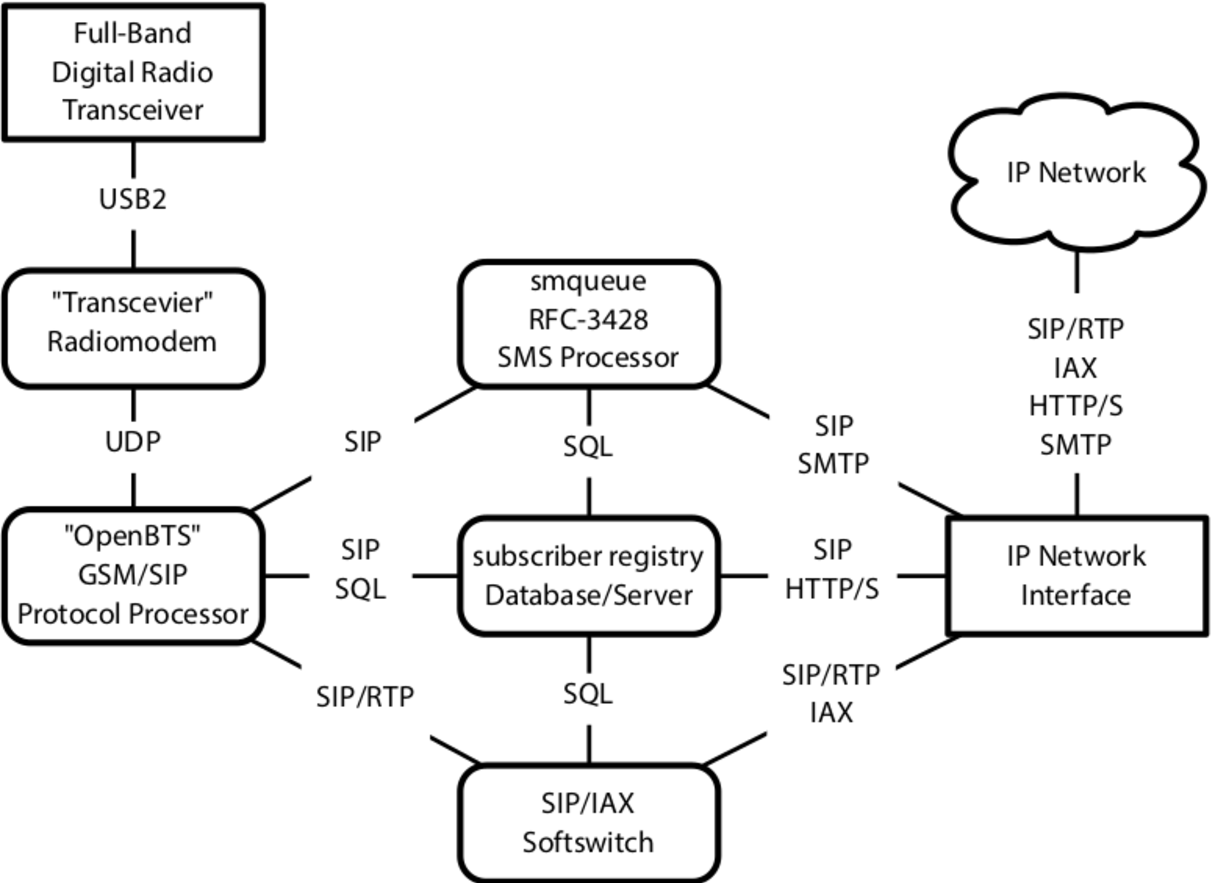
\includegraphics[width=\textwidth]{../images/btsSimple}
  \caption[Simplest OpenBTS network]{Components of the OpenBTS application suite 
  and their communication channels as installed in each
access point. Sharp-cornered boxes are hardware components.
Round-cornered boxes are software components \protect\cite{openbtsMan}.}
  \label{fig:btsSimple}
\end{figure}

\begin{figure}
  \centering
    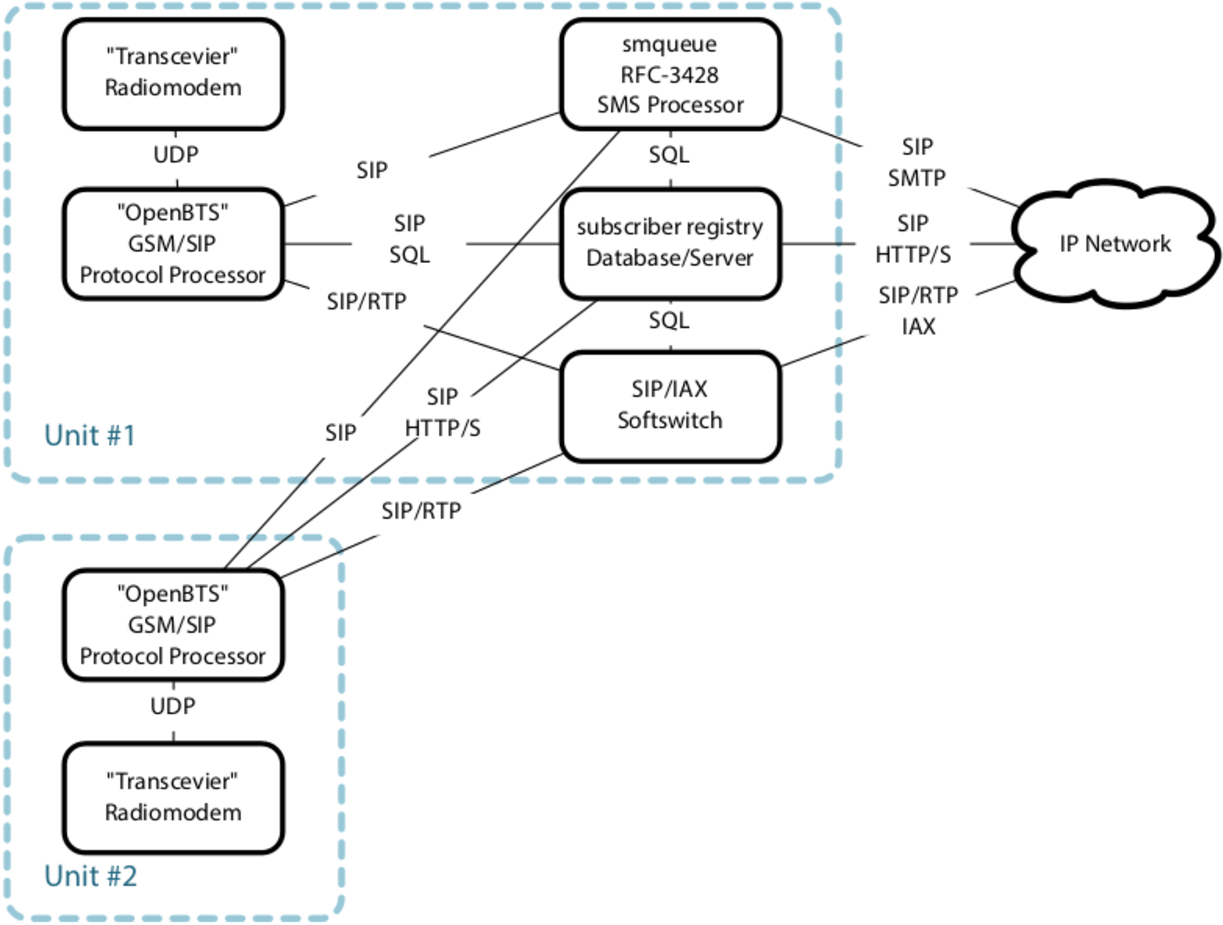
\includegraphics[width=\textwidth]{../images/btsLarge}
  \caption[OpenBTS network with two access points]{Two access points with unit 
  \#1 providing servers for both \protect\cite{openbtsMan}}
  \label{fig:btsLarge}
\end{figure}


\section{Asterisk}
Asterisk is an open source software implementation of a Private Branch
Exchange (PBX). Just like a real-world PBX, it allows attached phones to call
each other and to connect to other telephone services like the PSTN and the 
VoIP. It supports various VoIP protocols like Session Initiation Protocol (SIP),
H.323, etc. Besides VoIP protocols, it also supports traditional protocols 
like ISDN and SS7.

OpenBTS uses Asterisk to handle speech calls.

\section{Configuration of Asterisk}
Every phone operating in a GSM network has a Subscriber Identity Module (SIM)
card. Every SIM has an identifier called IMSI, which stands for International
Mobile Subscriber Identity.

Asterisk requires a unique name for each user. We use the IMSI
number for the name of every Asterisk user because the IMSI numbers are unique
to each GSM network user.

In order to register a SIM to an OpenBTS network, we need to edit two 
configuration files named \textsf{sip.conf} and \textsf{extensions.conf}. These
files are located in the folder \textsf{/etc/asterisk/} for a default 
installation of Asterisk.

We also have to update the database \textsf{sqlite3.db} located in
\textsf{/var/lib/asterisk/sqlite3dir/}.

\subsection{sip.conf}

The \textsf{sip.conf} file contains user device configuration for every user of 
the Asterisk system. This file contains a section for each user. A typical 
section is as follows:
\begin{verbatim}
[IMSI123451234512345]
callerid=1111
canreinvite=no
type=friend
context=sip-external
allow=gsm
host=dynamic
dtmfmode=info    
\end{verbatim}

The first line of each section is the device name (aka extension name in
Asterisk). We used the IMSI number of each SIM prefixed with the word ``IMSI''
just to ensure that the device names are unique to each user.

\begin{figure}
  \centering
    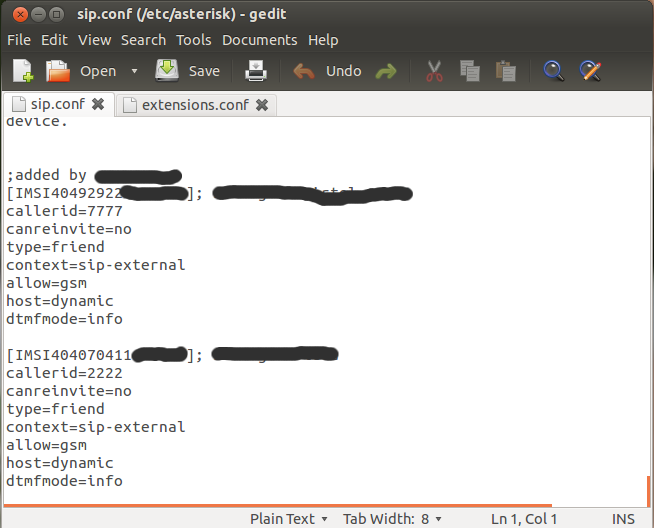
\includegraphics[width=0.9\textwidth]{../images/sip_conf}
  \caption[Screenshot - sip.conf]{Screenshot for \textsf{sip.conf}}
  \label{sip_conf}
\end{figure}

The \texttt{callerid} option sets dialling number of the device. The option
\texttt{host} is used for locating the user device in the network. Setting the
\texttt{host} as \textsl{dynamic} tells Asterisk that the user device will
update its location to Asterisk automatically and rids us of having to define 
the address statically. Otherwise we can define the addrsess of the device 
statically by setting the value of \texttt{host} to a specific IP address.

The option \texttt{type} is used to determine how the user is matched to the 
incoming request for a configuration entry. The \texttt{type} option can take any 
of the following values:
\begin{itemize}[noitemsep,topsep=0pt,parsep=0pt,partopsep=0pt]
    \item \textbf{peer -} The incoming request is matched using the IP
    address and the port number.
    \item \textbf{user -} The incoming request is matched using the 
    device name of the user.
    \item \textbf{friend -} The incoming request is matched on the name first,
    and then the IP address.
\end{itemize}

The requested user is handled by the dialplan in the \texttt{context} of the
device configuration. The dialplan configurations are contained in the
file \textsf{extensions.conf}. In our experiment, we have named the
\texttt{context} as \textsl{sip-external} and we have put all the phones used
in the experiment under this \texttt{context}. So, for each phone in our
experiment, Asterisk will be using the dialplan listed in the
\textsf{extensions.conf} file under the \texttt{context} of
\textsl{sip-external}.


The option \texttt{allow} controls the audio codecs that are allowed for the
phone.


\subsection{extensions.conf}

This file defines the dialplan followed for each user. The dialplan is a form
of scripting language. It contains instructions that Asterisk follows in 
response to some external triggers.

\begin{figure}
  \centering
    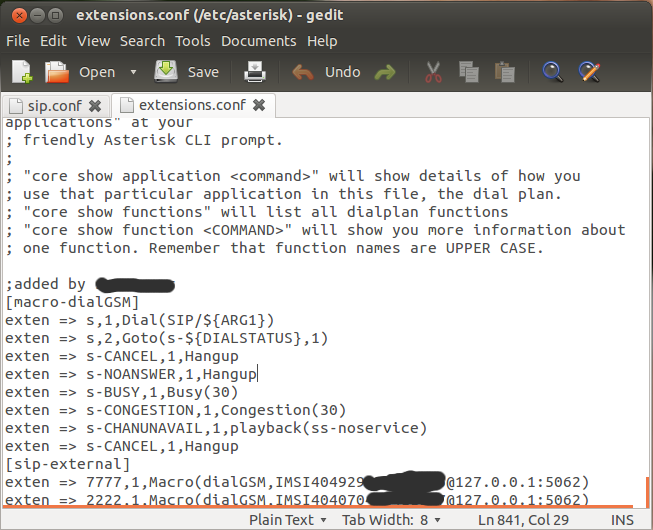
\includegraphics[width=0.9\textwidth]{../images/ext_conf}
  \caption[Screenshot - extensions.conf]{Screenshot for \textsf{extensions.conf}}
  \label{ext_conf}
\end{figure}
For our experiment, we added a macro to \textsf{extensions.conf} to avoid
having to repeat the same dialplan for each user/extension. The macro is
listed below:
\begin{verbatim}
[macro-dialGSM]
exten => s,1,Dial(SIP/${ARG1})
exten => s,2,Goto(s-${DIALSTATUS},1)
exten => s-CANCEL,1,Hangup
exten => s-NOANSWER,1,Hangup
exten => s-BUSY,1,Busy(30)
exten => s-CONGESTION,1,Congestion(30)
exten => s-CHANUNAVAIL,1,playback(ss-noservice)
exten => s-CANCEL,1,Hangup
\end{verbatim}

Then we configured each of our extensions under the \texttt{context} of 
\textsl{sip-external} as in the example that follows: 
\begin{verbatim}
[sip-external]
exten => 1111,1,Macro(dialGSM,IMSI123451234512345@127.0.0.1:5062)
exten => 2222,1,Macro(dialGSM,IMSI123451234512312@127.0.0.1:5062)
exten => 9999,1,Macro(dialGSM,IMSI123451234123412@127.0.0.1:5062)
exten => 5555,1,Macro(dialGSM,IMSI123412341234123@127.0.0.1:5062)   
\end{verbatim}


\subsection{sqlite3.db}

\begin{figure}
  \centering
    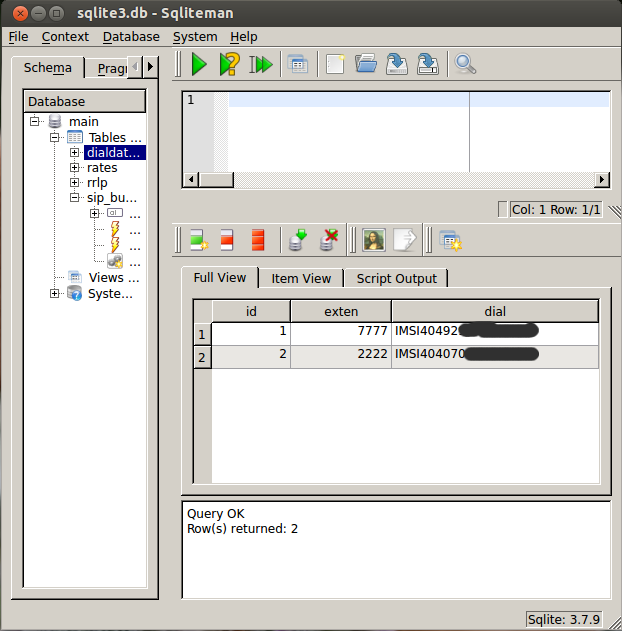
\includegraphics[width=0.9\textwidth]{../images/dialdata}
  \caption[Screenshot - dialdatatable]{Screenshot for \texttt{dialdatatable}}
  \label{dialdata}
\end{figure}

Asterisk also has a database in \textsl{sqlite} format storing all the 
\emph{caller id to device name} mapping data and the user device configuration
data. The table \texttt{dialdatatable} contains the mapping from each device
name to the corresponding caller id of the subscriber/user. The
\texttt{sip\_buddies} table on the other hand has all the user device 
configuration data already listed in \textsf{sip.conf}.

\begin{figure}
  \centering
    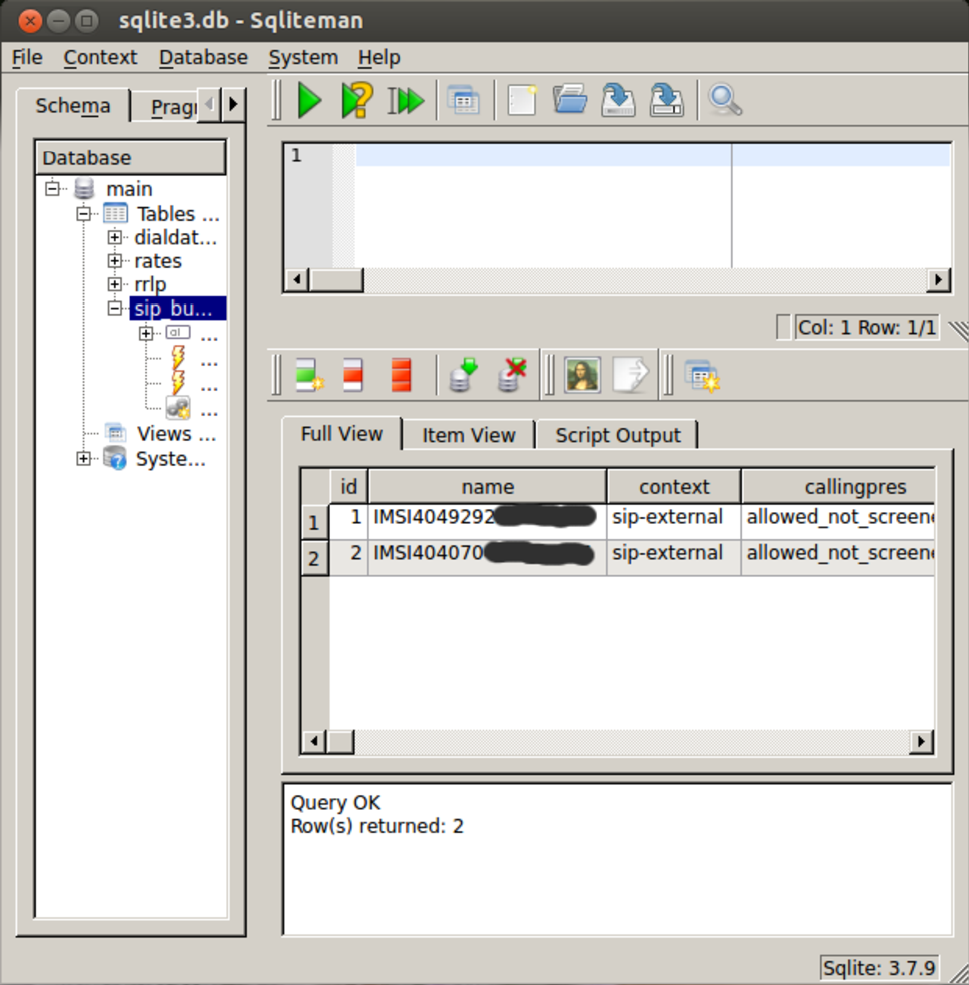
\includegraphics[width=0.9\textwidth]{../images/sipbuddies}
  \caption[Screenshot - sip\_buddies]{Screenshot for \texttt{sip\_buddies}}
  \label{sipbuddies}
\end{figure}


